\begin{figure}[h] %% zum drucken pdf verwenden
	\centering
  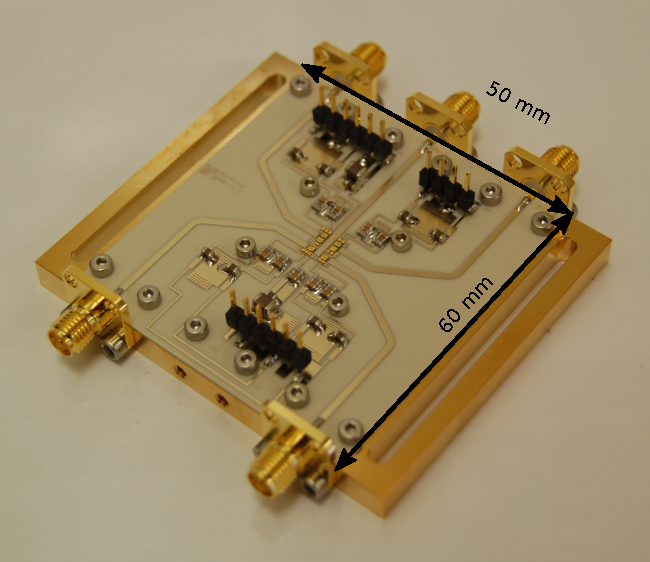
\includegraphics{Demonstrator_publish.pdf}
	\caption{Built demonstrator}
	\label{fig:Demonstrator}
\end{figure}
To the best of the author's knowledge, the worldwide first realised Riemann Pump in \gls{ab:gan} technology is presented in Figure \ref{fig:Demonstrator}.\\

In this work a new concept of digital to analog conversion is investigated, yielding an arbitrary waveform generator which can be used in the next generation of mobile communication.
For the development of this waveform generator, a proper concept is researched and simulated, a layout of the test circuit is developed and a first prototype is successfully built and measured.
The presented concept yields a waveform generator which is able to cover the frequency range from DC to \SI{6}{\giga \hertz} for baseband signals, which simulations confirmed.
As the signal generator handles digital data to generate the baseband signal it is working like a digital-to-analog converter.
With the help of this custom digital-to-analog converter, the actual conversion methods of digital to analog conversion are enhanced.
The first Riemann Pump in \gls{ab:gan} technology was built to prove the concept of a push-pull stage, providing a multi bit charge pump.
This multi chip solution is chosen to show the feasibility of generating different signals.
Simulations demonstrate some drawbacks and trade-offs regarding the power consumption, bandwidth limitation and some aspects are mentioned which influenced the signal quality.
In the design and realisation process custom drafts are developed to improve the heat transfer, while guarantee the proper functioning of the test circuit.
Some aspects are considered to reduce parasitic effects and undesired behaviour of the circuit.
After the assembly of the test circuit, different measurement concepts are prepared.
The four input ports required a special control strategy.
Further, a proper output measurement strategy is described to illustrate the results.
The successful measurement of the built demonstrator finishes the proof of the demonstrated concept.
At last a conclusion sums up the results of the presented work and give an outlook for further improvements.





%\textbf{Agenda}
%\begin{enumerate}
%	\item literature survey
%	\item adaption of push-pull concept from Maksimovic (Talk at Fraunhofer IAF 06/2015)
%	\item GaN25 \gls{ab:gan} parameter simulation [S-parameter,ON/OFF switching voltage]
%	\item determine load impedance [input of PPA - GaN25 \gls{ab:hemt}
%	\item determine dimension of transistors
%	\item tuning schematic parameter for optimal simulation (special freq?)
%	\item enhancement/extension of 1-bit push-pull to 3-bit push-pull stage
%	\item digital input control voltage
%	\item determine eight slopes of the current sources in schematic 3-bit resolution
%	\item Riemanncode generation with MatLab; minimizing error
%	\item control schematic with theoretical input [Riemanncode]
%\end{enumerate}
%\vspace{1cm}
%\textbf{Problems}
%\begin{enumerate}
%	\item frequency dependent load impedance
%	\item absence of p-type transistor makes it hard to efficiently switch the high side transistor in the Gbps range
%	\item the heat spreading on the chip and substrate is critical
%	\item energy consumption may be very high (mainly switching losses)
%	\item the absence of accurate current sources makes it very hard to get a defined slope for the switching transistors.
%	\item theoretical slope generation very inaccurate
%	\item theoretical slope generation via shorted load  (R = \SI{1}{\ohm})
%	\item \textit {$\rightarrow$ slopes ambiguous}?	
%	\item \textit{$\rightarrow$ riemanncode generation not possible}?                                                                                                                                                                                                                                                                                                                                                                                                                                                                                                                                                                                                                                                                                                                                                                                                                                                                                                                                                                                                                                                                                                                                                                                                                                                                                                                                                                                                                                             
%\end{enumerate}
%\vspace{1cm}
%\textbf{Question}
%\begin{enumerate}
%%	\item mmW band much higher BW,Datarate,Spectrum - why use the old fashioned frequency bands from DC to 6GHz instead of using a couple of GHz?
%%	\begin{itemize}
%%		\item carrier frequencies of modern telecommunication standards are in the range of DC to 6 GHz
%%		\item Signal generation is done for the bandwidth of 0..\SI{6}{\GHz}, after that it could be mixed up to higher frequency bands like \SI{47}{\GHz} to \SI{53}{\GHz}
%%	\end{itemize}
%	\item trade off between BW and losses
%	\begin{itemize}
%		\item higher bandwidth means higher switching speed means higher losses due to the fact that the losses increase linear with the switching speed
%	\item higher frequencies means higher attenuation (e.g. weather condition, like rain)
%	\end{itemize}
%\end{enumerate}

\newpage
\chapter*{Zusammenfassung}

In dieser Arbeit wird ein neus Konzept der Digital-Analog-Umwandlung untersucht, was zu einem Signalgenerator f\"uhrte, der in der n\"achsten Generation der mobilen Kommunikation verwendet werden k\"onnte.
F\"ur die Entwicklung eines solchen Signalgenerators wurden geeignete Konzepte untersucht und simuliert, ein Schaltungsentwurf entwickelt, ein erster Prototyp aufgebaut, dieser getestet und erfolgreich vermessen.
Das vorgestellte Konzept ergab einen Funktionsgenerator welcher in der Lage ist Signale im Frequenzbreich von \gls{ab:dc} bis \SI{6}{\giga \hertz} zu generieren, was Simulationen best\"atigten.
Mit Hilfe dieses Digital-Analog Wandlers wurde die Leistungsf\"ahigkeit bisheriger Methoden eindrucksvoll erh\"oht.
Die erste Riemann Pumpe in GaN Technologie wurde aufgebaut um das untersuchte Konzept einer Gegentaktstufe zu best\"atigen, was zu einer Ladungspumpe mit mehreren Bits f\"uhrte.
Um zu zeigen, dass verschiedene Signale generiert werden k\"onnen, wurden mehrere Chips verwendet.
Simulationen zeigten bereits einige Nachteile und Trade-offs was insbesondere den Energieverbauch und die begrenzte Bandbreite angeht.
Ausserdem werden einige Gesichtspunkte erl\"autert, die die Qualit\"at des generierten Signals beeinflussen.
Im Schaltungsentwicklungsablauf werden spezielle Entw\"urfe vorgestellt, die das Problem der W\"armeabfuhr verbessern und gleichzeitig das korrekte Funktionieren der Schaltung sicherstellen.
Einige Aspekte wurden untersucht um parasit\"are Effekte zu reduzieren und unerw\"unschtes Verhalten der Schaltung zu vermeiden.
Nachdem die entwickelte Schaltung konkret aufgebaut wurde, wurden verschiedene Messaufbauten vorbereitet.
Die vier Eingangsports der Schaltung ben\"otigten eine spezielle Kontrollstrategie.
Weiterhin ist eine geeignete Strategie beschrieben, die das korrekte Messen am Ausgang erm\"oglichte.
Das erfolgreiche Messen der aufgebauten Testschaltung erbringt den Machbarkeitsnachweis von dem vorgestellten und entwickelten Konzept.
Als letztes fasst die Schlussfolgerung alle wesentlichen Ergebnisse dieser Arbeit zusammen und ein Ausblick f\"ur weitere Entwicklungsm\"oglichkeiten wird gegeben.
